\chapter{Основные сведения о дальнейших аспектах оптимизации}
\section{Общие сведения об итераторах планов}

\subsection*{Резюме занятия}
\begin{itemize}
	\item SQL Server использует много различных методов доступа к данным. 
	\item SQL Server использует разные алгоритмы соединений и статистической обработки. 
	\item Не существует "хороших" и "плохих" итераторов. Любой итератор может подходить наилучшим образом для конкретного запроса и конкретных данных. 
\end{itemize}

\subsection*{Закрепление материала}

\begin{figure}[h!]
	\begin{center}
		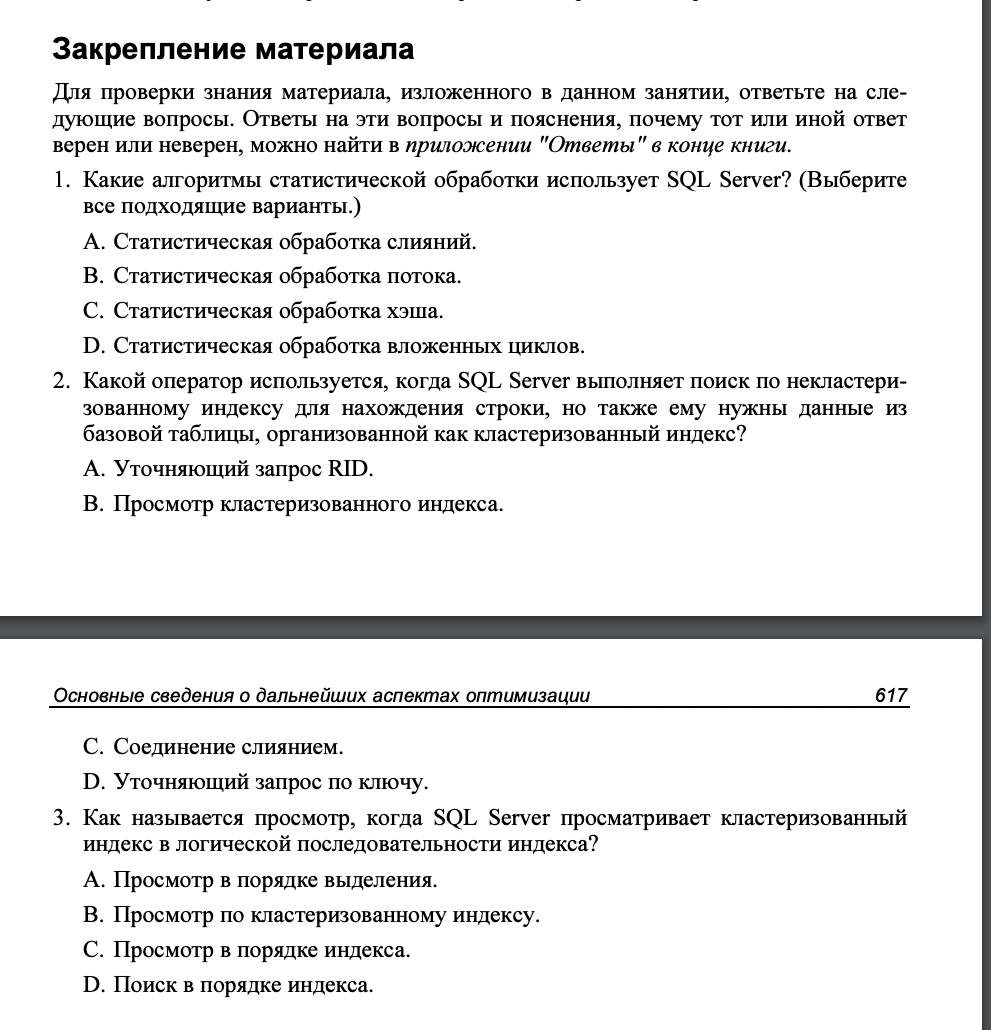
\includegraphics[width=0.7\textwidth]{img/zakrep48.png}
	\end{center}
	\captionsetup{justification=centering}
\end{figure}
\newpage

\subsection*{Ответы}

\begin{figure}[h!]
	\begin{center}
		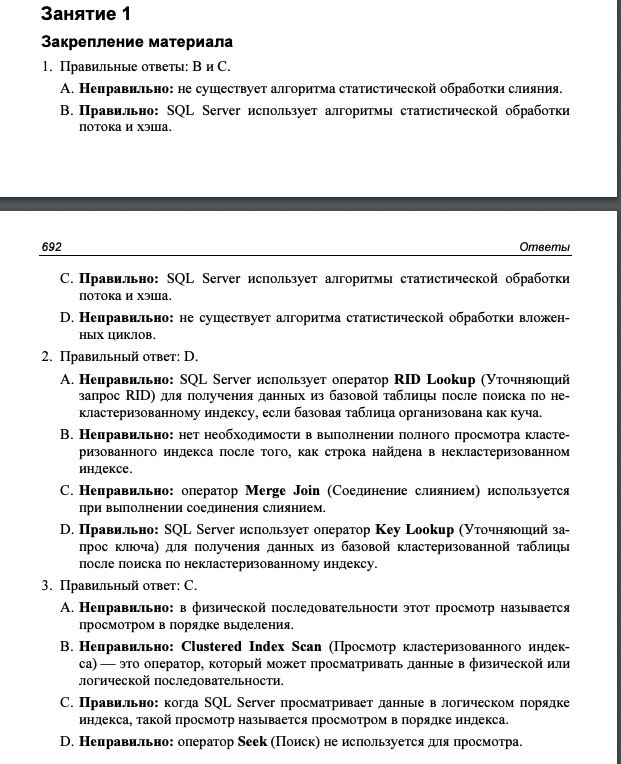
\includegraphics[width=0.6\textwidth]{img/eans48.png}
	\end{center}
	\captionsetup{justification=centering}
\end{figure}
\clearpage



\section{Использование параметризованных запросов и пакетных операций}

\subsection*{Резюме занятия}
\begin{itemize}
	\item SQL Server выполняет параметризацию запросов для улучшения повторного использования планов выполнения. 
	\item Вы можете выполнить параметризацию запросов самостоятельно. 
	\item Режим пакетной обработки, который появился только в SQL Server 2012, может
	значительно повысить производительность запросов к хранилищам данных,
	особенно снижением использования ЦП. 
	\item Пакетная обработка хорошо совмещается с индексами columnstore. 
\end{itemize}


\subsection*{Закрепление материала}

\begin{figure}[h!]
	\begin{center}
		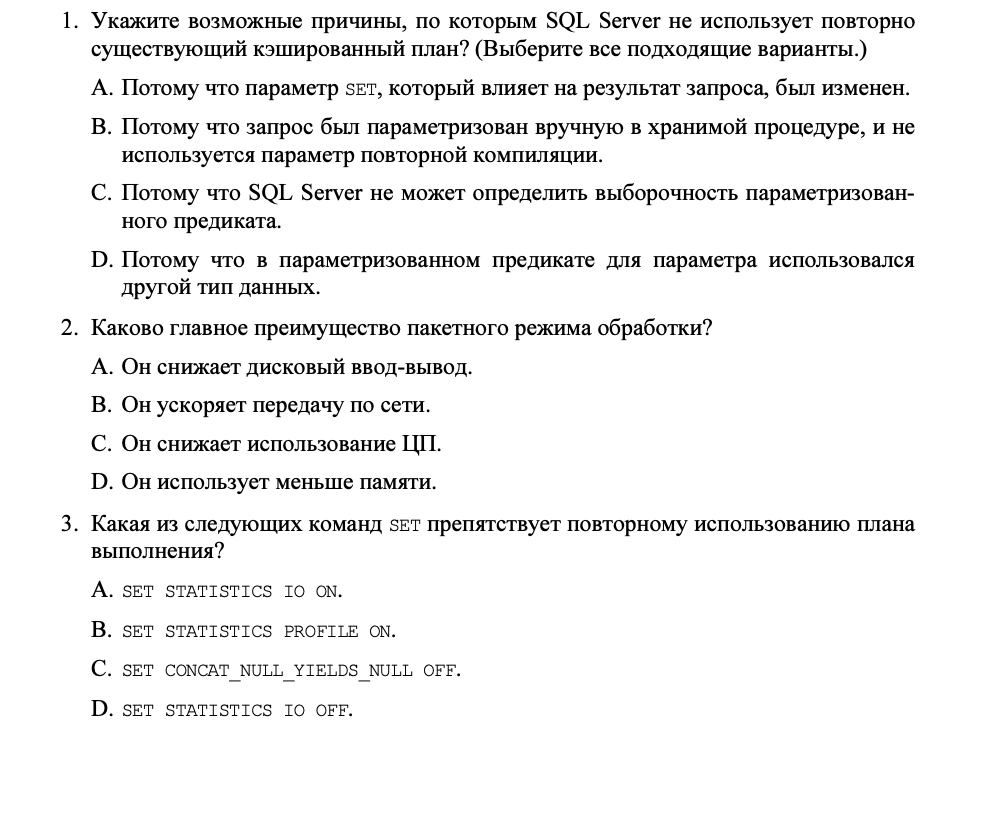
\includegraphics[width=0.9\textwidth]{img/zakrep49.png}
	\end{center}
	\captionsetup{justification=centering}
\end{figure}
\clearpage	

\subsection*{Ответы}

\begin{figure}[h!]
	\begin{center}
		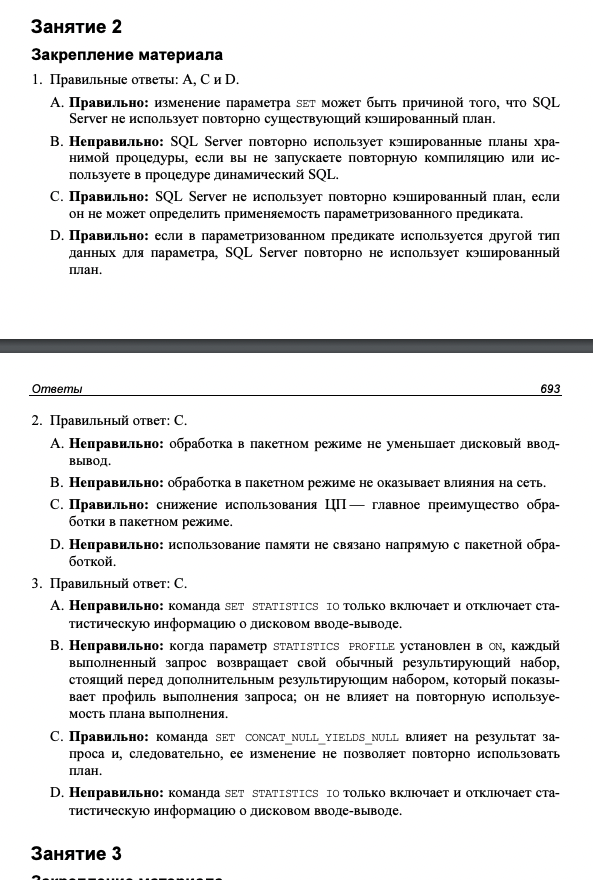
\includegraphics[width=0.9\textwidth]{img/ans49.png}
	\end{center}
	\captionsetup{justification=centering}
\end{figure}


\newpage
\subsection*{Упражнения}

\begin{figure}[h!]
	\begin{center}
		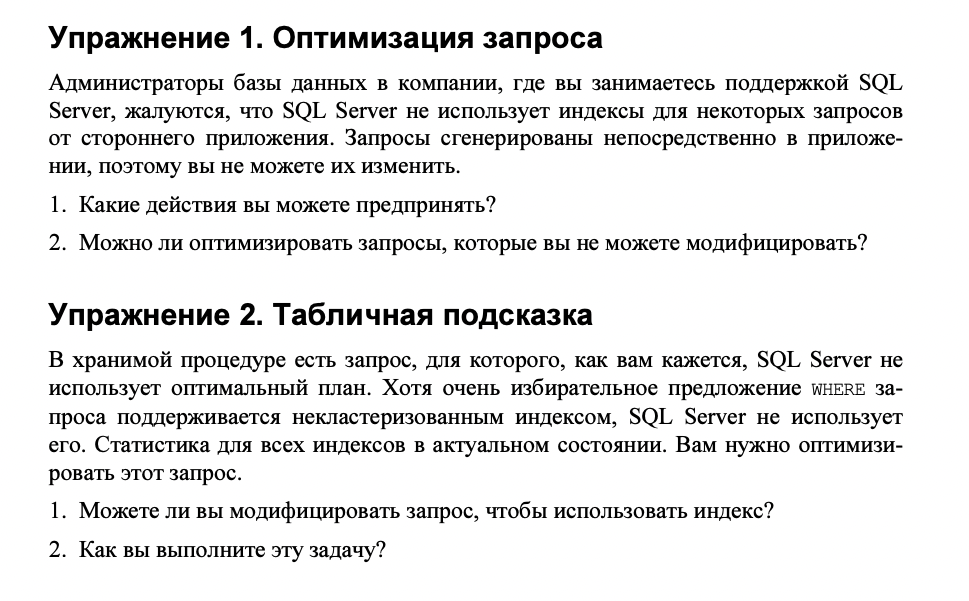
\includegraphics[width=0.6\textwidth]{img/ex50.png}
	\end{center}
	\captionsetup{justification=centering}
\end{figure}

\subsection*{Ответы}

\begin{figure}[h!]
	\begin{center}
		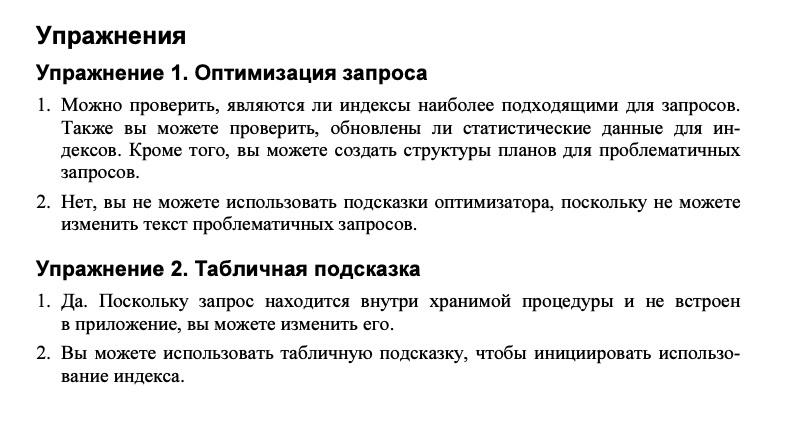
\includegraphics[width=0.6\textwidth]{img/eans50.png}
	\end{center}
	\captionsetup{justification=centering}
\end{figure}